\documentclass{article}

\usepackage{graphicx}
\usepackage{listings}

\title{Homework 4}
\author{Mitchel Fields}
\begin{document}

\maketitle

\begin{itemize}
	\item [\textbf{Problem 1}]\hspace{0pt}\\
	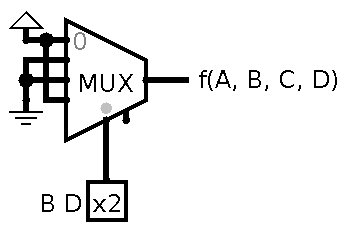
\includegraphics[scale=0.5]{hw4-1a}\\
	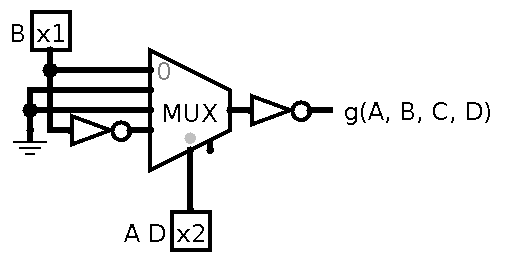
\includegraphics[scale=0.5]{hw4-1b}

	\item [\textbf{Problem 2}]\hspace{0pt}\\
	\lstinputlisting[language=Python]{homework4.py}

	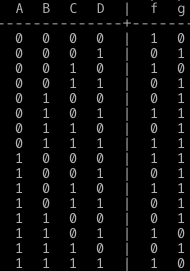
\includegraphics[]{hw4-2}

	\item [\textbf{Problem 3}]\hspace{0pt}\\
	The circuit is not a latch. When initialized, the ciruit will default to the following state:\\
	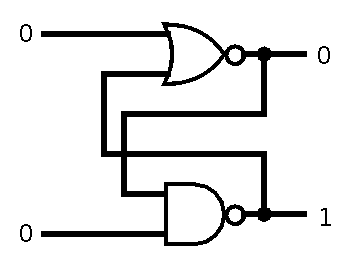
\includegraphics[scale=0.5]{hw4-3a}

	And cannot be changed:\\
	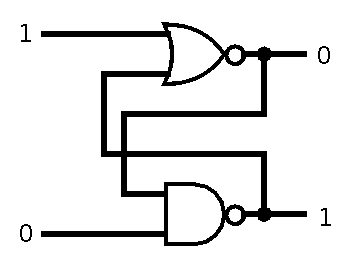
\includegraphics[scale=0.5]{hw4-3b}\\
	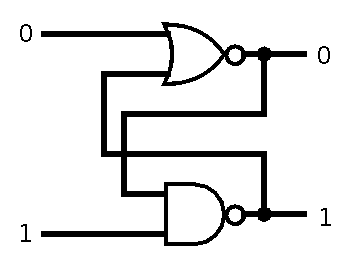
\includegraphics[scale=0.5]{hw4-3c}\\
	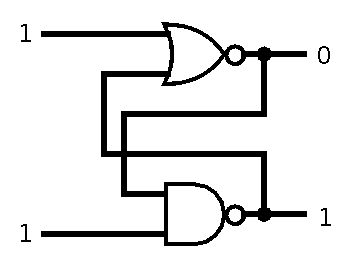
\includegraphics[scale=0.5]{hw4-3d}

	\item [\textbf{Problem 4}]\hspace{0pt}\\
	A latch can be created with the first gate the following way (the square gates represent the AND with an inverted input):\\
	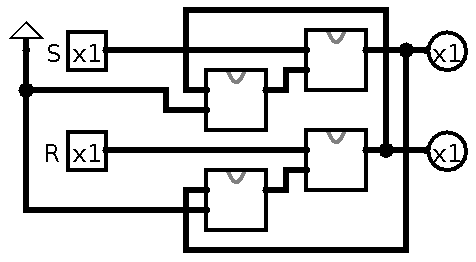
\includegraphics[scale=0.5]{hw4-4a}

	The XOR with an inverted input cannot be made into a latch. It can only implement an inverter and, through that, an XOR and XNOR. These gates cannot be arranged to be equivalent to a NOR or a NAND gate. They cannot be made to pass in 3 states and block in 1 and, thus, cannot form a latch. 

\end{itemize}

\end{document}